\section{Which Differences Persist When Inputs Change?}
\label{sec:stability}

\subsection{A Teaching Habit Need Not Appear in Every Reply}
Past behavior can help predict a model's next response even when it does not
repeat the same action every time. M3 agrees with itself on whether to invite
reasoning in only 57.8\% of 128 matched input pairs (95\% source-bootstrap
interval 50.0--66.4\%). High agreement can also reflect repeated absence:
DeepSeek and Doubao agree on whether to invite reasoning in over 90\% of
repeated responses, but none of their few invitations appear in both responses. They agree perfectly on answer
revelation because they always reveal an answer in this sample.

Agreement therefore needs to be read alongside how often each action occurs
and whether earlier responses help predict later ones
(Appendix~\ref{app:confirmation-details}).
Appendix~\ref{app:materials-examples} illustrates the codes on matched replies.

\subsection{Past Behavior Helps Predict New Responses (RQ2)}
Knowing the model's usual behavior improves prediction of all three actions
on new problems, compared with knowing only the subject and student state.
Brier loss decreases by 0.091 for answer revelation, 0.130 for reasoning
elicitation, and 0.020 for acknowledgement; all three gains pass the six-test
Holm correction. Thus, models' previous teaching choices provide information
that the scripted educational context alone does not supply.

Knowing how each model responds to student cues further improves acknowledgement
predictions over its usual rate within a subject. The same comparison gives no
clear additional benefit for revelation or elicitation. Full estimates and
uncertainty intervals appear in Appendix Tables~\ref{tab:absolute-losses}
and~\ref{tab:primary-tests}.

A predictor based on the length and formatting of training responses makes larger errors
than the model-default predictor for all three actions
(Appendix Table~\ref{tab:absolute-losses}). These two style measures do not
match the predictive performance of model defaults. Richer style measures may
do better, and the comparison does not identify a causal effect of model identity.

\subsection{Prediction Under New Student Wording (RQ2)}
\label{sec:cue-results}

When students express themselves differently, the original model defaults still
help predict whether tutors give answers or invite reasoning. For acknowledgement,
the extra benefit of knowing each model's response to student cues is lost.
This benefit remains positive when we collect new replies using the original
wording during the same period. The contrast weakens an explanation based only on a general loss of predictive
value over time. Figure~\ref{fig:expression-transfer}
shows the estimates and uncertainty; Appendix Table~\ref{tab:cue-primary}
gives all six tests and Appendix~\ref{app:cue-transfer} the paired contrasts.

\begin{figure}[t]
\centering
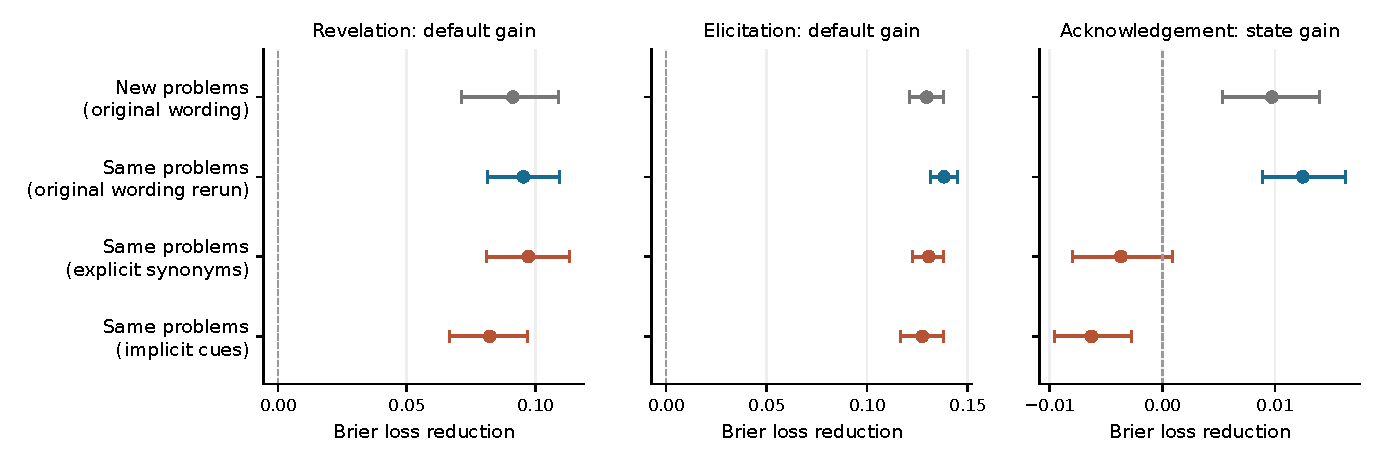
\includegraphics[width=\linewidth]{figures/expression_transfer.pdf}
\caption{Transfer depends on what is changed. The initial test uses
new problems with the original wording. The three follow-up conditions use
those same 32 problems and the earlier predictions. Default gains for giving answers and
inviting reasoning remain positive, while the state gain for acknowledgement
is no longer positive under new wording. Bars are source bootstrap 95\%
intervals conditional on frozen fits, not four independent replications or
simultaneous intervals. Horizontal scales differ by panel.}
\label{fig:expression-transfer}
\end{figure}

The acknowledgement gains have the same sign pattern when each annotator's labels
are used separately and when each generating model is left out, although some
intervals include zero. These checks reuse the same responses. The result
concerns prediction: models still acknowledge feeling or difficulty at different
rates for contrasting student cues. It does not mean that models stop responding to
student cues. The implicit condition also changes more than affect wording.

\paragraph{Alternative explanations.}
Losing an advantage over a baseline does not always mean making larger errors.
Under explicit synonyms, the cue-based predictor's own loss improves slightly,
yet it no longer outperforms the baseline. Under implicit cues, its own loss
also worsens. Further checks show that a common change in acknowledgement
frequency cannot explain the contrast, and the tested logistic recalibrations
do not restore a positive gain. These follow-up analyses narrow the explanations
without identifying a unique mechanism
(Appendices~\ref{app:cue-diagnosis}--\ref{app:cue-calibration}).

In the additional classmate control, changing a classmate's quoted feelings changes
acknowledgement rates even though the current student remains calm. Selected
examples show this can happen when the model correctly distinguishes the two
students' feelings. The contrast alone therefore does not establish confusion
about whose feelings are being expressed (Appendix~\ref{app:cue-transfer}).


\subsection{Useful Predictions Do Not Require Unchanged Action Rates}
A model's action rates can change while its earlier behavior still helps
predict new responses. Neutral role paraphrases produce some observed shifts,
and our sample is too limited to establish equivalence
(Appendix~\ref{app:confirmation-details}). The transfer tests show that previous
behavior remains informative under the tested changes. They do not show that
rates or model rankings stay fixed. Default and state gains also compare
different predictors, so their sizes cannot be read as a common stability
score. Persistence across provider updates remains untested.

\subsection{Checking Dependence on Annotators, Models, and Answer Errors}
The main pattern holds across eight sets of annotator labels: model defaults
improve prediction, and cue-specific responses add value mainly for
acknowledgement. Resampling training sources and checking missing codes
preserve this pattern. These checks reduce concern that the findings depend
on one coding choice, but do not establish that the labels are correct
(Appendix~\ref{app:confirmation-details}).

The strength of the differences depends on which models are compared.
Removing GLM substantially reduces default gains for revelation and elicitation.
Removing M2.7 leaves a small default acknowledgement gain whose interval spans
zero. The result for all five models therefore need not hold equally strongly for every
subset of models.

Default gains and the acknowledgement state gain remain positive after excluding
matched response groups flagged for answer errors. However, reviewers often
disagree about these errors. The screen cannot guarantee correct retained
answers or rule out differences in task ability
(Appendix~\ref{app:content-results}).
